\documentclass[a4paper,oneside]{report}

\usepackage{amsmath}
\usepackage{amssymb}
\usepackage{caption}
\usepackage[english]{babel}
\usepackage{fancyhdr} 
\usepackage{float}
\usepackage{multirow}
\usepackage[pdftex]{graphicx}
\usepackage{listings}      
\usepackage{pdfpages}
\usepackage{setspace}
\usepackage{url}
\usepackage{wrapfig}

\lstset{language=C,
numberstyle=\footnotesize,
%basicstyle=\ttfamily\footnotesize,
basicstyle=\footnotesize,
numbers=left,
stepnumber=1,
frame= lines,
breaklines=true}

\makeatletter


%
% Some custom definitions
%

% add horizontal lines
\newcommand{\HRule}{\rule{\linewidth}{0.5mm}}
\newcommand{\HRuleLight}{\rule{\linewidth}{0.1mm}}

% custom part page
\def\part#1#2
{
	\par\break
  	\addcontentsline{toc}{part}{#1}
	\noindent
	\null	
	\HRuleLight\\[0.0cm]
	\vspace{20pt}	 
	\begin{flushright} 		
  	{\Huge \bfseries \noindent #1}\\
  	\vspace{30pt} 
	\begin{minipage}{0.85\textwidth}
		\begin{flushright}
		{\large \noindent #2}
		\end{flushright}
	\end{minipage}\\[0.75cm] 
	\end{flushright} 		
	\thispagestyle{empty}
	\break
}

% chapter header
\renewcommand{\@makechapterhead}[1]
{\vspace*{50\p@}{
	\parindent \z@ \raggedright \normalfont
	%\huge \bfseries \thechapter. #1
	\huge \bfseries #1
	\vspace{20pt}}}

\setcounter{secnumdepth}{-1} 
\onehalfspace
\oddsidemargin 1in 
\oddsidemargin 0.6in 
\topmargin -0.3in
\setlength{\textwidth}{14cm}
\setlength{\textheight}{23cm}
\lstset{language=C} 

\begin{document}

%
% Cover page
%
\begin{titlepage}
\begin{center}

\Huge Donald Nute's VWorld\\ 
\huge \emph{Bumble 2.0}

\HRuleLight\\[0.5cm]

\begin{minipage}{0.45\textwidth}
	\begin{flushleft}\large
		\emph{Author:}\\
			\textbf{James P. \textsc{Spencer}}\\[0.27cm]
			Computer Science (Games)
			Student Number: 08809130
	\end{flushleft}
\end{minipage}
\begin{minipage}{0.45\textwidth}
	\begin{flushright}\large
		\emph{Author:}\\
			\textbf{Thomas J. \textsc{Taylor}}\\[0.27cm]
			Computer Science (Games)
			Student Number: 08813043
	\end{flushright}
\end{minipage}\\[0.75cm] 

\HRuleLight\\[0.2cm]

\large School of Computing, Engineering and Mathematics\\ \textbf{University of Brighton}

\vfill
\huge Documentation\\
\large April, 2012\\

\end{center}
\end{titlepage}

% reset page count
\setcounter{page}{1}

\section{Introduction}

At the beginning of the module, we were presented with Donald Knute's VWorld: a simple 2D sandbox game environment written in the Prolog logic programming language.

The game world itself is represented as a 2D grid structure, and can consist of a number of different levels (or rooms) interconnected with doors. Each level is filled with a number of different objects, ranging from impassable walls, to collectibles such as health power ups (fruit) and weapons (a sword), to NPCs such as snails and hornets, which try to hinder the player's progress by inflicting damage or blocking their path. 

The VWorld game framework we were given was already set up to deal with the more low-level functionality such as the user-interface elements and graphical display and loading and initialising the game. A number of different behaviours were also predefined for the non-player characters (NPCs). For example, the NPCs were able to move around the level (and guard objects in the case of Dragons and witches). As mentioned, the snails follow the player in an attempt to block their path, and the hornets attack the player, inflicting damage. 

The main protagonist of the game is Bumble: an AI character who finds himself in the mysterious realm of VWorld. He must have his wits about him at all times in order to survive this treacherous land. Bumble is given a number of tools to aid him in his fight against evil, such as a sword, a shield and bugspray. These items are scattered about the level, and must be searched down before they can be used.

\section{Aims and Objectives}

We were given a lot of freedom with this project in terms of the actual requirements. As there is no real `aim' in the VWorld game, we were left to our own devices to develop the system as we saw fit. The guidelines for the project were appropriately open-ended:

\begin{quotation} 
Modify aspects of [\emph{VWorld}] to make the behaviour of the actors (including Bumble) more 'interesting' than it is at the end of the formal workshops 
\end{quotation}

To give us some idea as to which areas we could develop, we were given a number of test level maps, which are designed in such a way as to encourage certain behaviour. For example, some of the test levels included the `bird' character who must be caught to complete the level. Catching the bird requires Bumble to collect `birdseed' located somewhere in the level, and so it can easily be seen that some sort of objectives are required for Bumble to succeed in such levels. Similarly, some levels have locked doors which require specific keys to enter.

There were a number of different angles from which we could approach this problem. Our first goal with this project was to simply increase Bumble's survival rate, as we felt that this was needed before any other aspects of the game could be improved. As a part of this objective, we also wanted to fix a number of issues with the basic Bumble and VWorld framework. Moving on from these small incremental changes, we wanted to implement some sort of search algorithm which Bumble could use in combination with his dynamic map of the world to find objects he had previously seen.

We used the test levels to create a basic 'specification' of the kind of behaviour we wanted Bumble to exhibit:

\begin{itemize}
	\item Some form of search
	\item Refine Bumble's strength/damage system
	\item Implement some exploration
\end{itemize}

Our overall goal was to iterate rather than to innovate, by developing the existing behaviour, fixing existing issues, and by implementing more incremental changes.

\section{Basic Bumble}

To start us off, we were given a very basic Bumble which we could use as a starting point for our development. The original Bumble was able to randomly explore the environment, but little else. In the tutorial sessions, we began to develop some basic behaviour for Bumble. By the end of the tutorials, Bumble was able to:

\begin{itemize}
	\item Randomly navigate the world
	\item Pick up any interesting/desirable objects he was stood next to
\end{itemize}





By the end of the tutorials, Bumble was able to move around the game world, and build a 'map' of where certain objects were located as they were found. 


Bumble has a few basic stats which are updated as he roams the level: strength, which decreases as Bumble moves around the level and can be replenished with tasty apples, and damage, which is incremented if Bumble is attacked. Bumble dies if either his strength reaches 0, which means he is unable to move, or if his damage reaches 100\%.

Bumble also had a few basic rules to help with his survival in the dangerous world. These rules are used to ascertain whether Bumble is hungry or hurt based on his current strength and damage levels. This information is then used to point Bumble in the direction of any power-ups as appropriate. This behaviour was quite naive, as Bumble would only move towards power-ups in his immediate vicinity (i.e. less than 2 squares away). In addition to this, Bumble also collected any `interesting' or `desirable' objects that he was standing next to.

As it was, Bumble's behaviour was still very naive. Bumble only considered objects which were very close by (i.e. within a two square `radius'). Although we had a map of the world which Bumble created dynamically as he explored the world, nothing was done with this map. The way Bumble treated objects in the game was also very simplistic: 'interesting' or 'desirable' objects were only picked up if Bumble was stood directly beside them, and Bumble had no real decision-making process with regards to picking up fruit or crosses. As it stood, Bumble would simple become 'hungry' when his strength dropped to a certain level, and 'hurt' when his damage exceeded a set value; there was no reasoning behind his decisions. Additionally, 

; he was only able to react to objects he was close to, despite the fact that a map was dynamically generated as Bumble explored the level. There was also no real 'method' behind Bumble's navigation, he simple wandered around randomly. Bumble also had no sense of any 'objectives' in the level. For example, he had no idea that in order to catch the bird, he first needed some birdseed. There were also a number of small bugs in the existing system which hindered his progress. 

\section{Modifications}

One of the key elements in our strategy was the smaller, more incremental changes and bug-fixes to the original system. While these may seem fairly insignificant, we feel that they actually contributed greatly to Bumble's appearance of intelligence, and the overall `believability' of VWorld as a game.

One of the first changes we made was to add extra predicates to allow Bumble to spot interesting and desirable objects from two squares away, and move towards them (as he does with the tree/cross). This obviously meant that Bumble was more likely to pick up these useful objects whilst exploring. We also ordered these predicates in a logical was to reflect the priority that Bumble would use. These priorities for removable objects (including crosses and trees) is given below:

\singlespace
\begin{enumerate}
	\item Eat fruit
	\item Push tree
	\item Push cross
	\item Collect desirable object
	\item Collect interesting object
	\item Catch bird \footnote{If Bumble is next to a bird and has birdseed, he can catch the bird. We discovered a bug (or maybe a feature?) whereby the bird was afraid of the bugspray, so Bumble also needed to drop the bugspray before catching the bird}
	\item Move towards cross
	\item Move towards tree
\end{enumerate}
\onehalfspace



The hornets follow Bumble upon spying him.

Bumble no longer flees if in possession of the shield/sword

Fixed a bug whereby Bumble could get stuck alternating between two interesting objects (e.g. tree/cross)

Hornets no longer cause injury if Bumble's in possession of the bugspray. Also, the bugspray now actually works.

Fixed a bug whereby Bumble could get stuck in a corridor 1 sq wide (see castle2.vw). 
If there was an interesting/ desirable object at the end of the corridor, Bumble would try to go west, but would simple stay in the same sqaure. There's now a check to see if Bumble already attempted the same move, if so, he moves randomly.

A map of the entire level is built. When Bumble goes through a door, an extra square is added in the appropriate direction to account for the wall in-between the levels. 

As removable items are taken by Bumble, they are also removed from the map.

\section{New Features}

In addition to the bug-fixes and modifications that we made to the system, we also implemented a few new features. These are outlined in this section.

\subsection{Search}

Search is a major area of game AI as it helps add realism and efficiency to agents movements. Implementing some form of search algorithm was key to the success of Bumble in the game; he needed some way to be able to seek out previously-visited resources as and when he needed them. For instance, if he is hungry he should be able to negotiate to a tree or any food he has seen. 

We have experimented with a few types of search, using workshops 4 and 5 as a starting point. In our initial investigations, we explored the use of breadth and depth first search. After further investigation, we decided that neither of these types of search were suited for VWorld (or indeed games in general), primarily due to the fact that they have a very poor worst case performance. Additionally, the paths they produce are often far from optimal, and rarely 'natural'. Agents which use `natural looking' paths are key to the believability of the game. 

For this reason, we explored the use of heuristic-based search in our game. We primarily looked at greedy and A* search although it should be noted that we did consider several other search methods that could give even more naturalistic approaches such as Theta* however we decided that implementing this would be non-trivial (exacerbated by our inexperience with using Prolog), and of little value due to the grid based system present in VWorld. Overall, implementing search proved to be the most challenging aspect of development, and was the main reason that we have been unable to implement A*, instead sticking with the slightly simpler greedy search.  

At the highest level, our search functions by looking for a path to an object given a current condition. Calling the search predicate will generate a path to the desired object provided that it is contained in Bumble's current map of the world.  There are however issues that can arise in this process. One issue arises when another agent such as a hornet blocks Bumble's next step. In this situation, he will have to avoid the desired cell and move into one adjacent to it. This is handled by defining a list of predicates for adjacent cells. 

For example, if the desired cell is north-west of Bumble's current position, and it is blocked by a hornet, Bumble will move to either north or west if he can. If Bumble is unable to even move to an adjacent cell, he simply moves randomly. In any case, Bumble's path will now be incorrect, so it is erased. This is essentially a simple form of collision avoidance, and could be extended further through the use of ray-casting, similar to that of the Open Steer C++ library.

Our implementation of greedy search is based on the code provided for the workshop. There were several issues with this code, and for this reason we have made some minor adjustments. The main change we have implemented is to a counter to count the number of times the search recurses. This is a deliberate `hack' which we deemed to be necessary to prevent heap overflow errors, and game crashes. We invested hours trying to find and debug the underlying cause of this issue, but without any success, hence our less-than-perfect solution. One improvement we did make which slightly alleviated this bug was to make sure that Bumble checked if he was following a path before anything else. We found that in some levels, Bumble would be too cautious around the NPCs, trying to flee even if he was following a search path.  Although this bug does not prevent search from functioning, it does mean that the application is unlikely to run for a great deal of time, as Bumble will often become `stuck' between walls and other NPCs, causing death die-by-starvation. Overall this bug is the primary barrier to the success of our system and in resolving it we feel that we would have had a far more impressive AI system. 

\subsection{Fuzzy-Inspired Reasoning}

We also wanted to apply some fuzzy reasoning to the Bumble's states (i.e. hungry and hurt). The idea behind being that Bumble could prioritise which power-up was needed based on whether he was more hungry, or more hurt. We initially implemented the traditional `fuzzy' style of reasoning, but found that the probabilistic element didn't really result in the behaviour that we wanted, as it caused very unpredictable and unrealistic behaviour. For this reason, we instead decided to create a fuzzy `inspired' method of reasoning. We did this by adding extra levels of hurt and hunger (starving, very hungry, medium hungry, not hungry etc.). Using these extra levels meant that we were then able to have more control over when Bumble would go for crosses and fruit. This was a particularly important issue after we implemented the search, as Bumble's state could change mid-path. After adding these new states, we created new predicates $eat(\_,\_)$ and $heal(\_,\_)$. Below is an example of this:

\begin{verbatim}
eat(_,_):-
    hungry_status(starving).

eat(_,_):-
    \+ hurt_status(critically_hurt),
    hungry_status(very_hungry).

eat(_,_):-
    hungry_status(medium_hungry),
    \+ hurt_status(medium_hurt),
    \+ hurt_status(small_hurt).
\end{verbatim}
	
This predicate is used to determine whether Bumble should try to eat or not. As can be seen from the code, Bumble will always eat if he is starving, but will prioritise his health if he is $critically_hurt$. In the final predicate, we can see that Bumble will only eat if he is $medium_hungry$ when his health is high (i.e. not $small_hurt$ or $medum_hurt$).

\subsection{Exploration}

The final additional feature that we added was a way for Bumble to explore the map in a more effective way than simply randomly walking around. To do this, we created an $exploration/0$ flag which stored whether or not Bumble should `explore' the world. This flag is based on whether or not Bumble can see any unvisited squares in his immediate vicinity (i.e. within a one square `radius'). For this to work, we also needed to add a list of visited squares stored as (X,Y) coordinates ($visited/2$). As Bumble explores the world, he adds the squares he visits to the list. Exploration mode is also enabled and disabled based on Bumble's current strength and damage values; this discourages Bumble from exploring unknown terrain if he's injured or hungry. Including this exploration mode means that items are found as quickly as possible. It also means that Bumble spends less time moving around randomly at the beginning of the game; a lot of time (and strength) was often wasted due to Bumble running around in illogical circles in areas that he had already visited.

The method by which Bumble explores the environment is very naive. It simply looks for unvisited squares around Bumble in the following order: east, north-east, north, north-west, west, south-west, south, south-east. Exploration could be greatly improved if some algorithm was used which allows Bumble to explore the map in a more logical and methodical way such as the wall-follower algorithm.

\section{Team Development}
	
As we were working in a pair, it was very important to ensure that we put some measure in place to make sure that we could collaborate efficiently without causing any corruption by editing the same file at the same time. This was particularly important for this project, as we were only really working from a single source file. Using source control also means that we were also creating incremental backups of the project, which was very useful to compensate for data loss.

We decided to use the Git version control system for this. Using Git, we made use of the branching feature, which allowed us both to create a separate `branch' of the code, which we could then work on two implement a new feature. After the feature had been implemented and tested, we could then merge that branch back into the main branch. This development process worked well.

We used Github to host our Git repository. As a side product of this, we were also able to make use of Github's 'Issues' feature, which allows all team members to add 
	
\section{Testing and Analysis}

We have utilised the set of test maps supplied with bumble to evaluate the effectiveness of our solution. In this experimentation we work with the assumption that if bumble survives more than 5000 moves he will live infinitely.
	
	\subsection{Bird One}

		\begin{figure}[h!]
		  \caption{Screenshot of bumble compleating bird one.}
		  \centering
			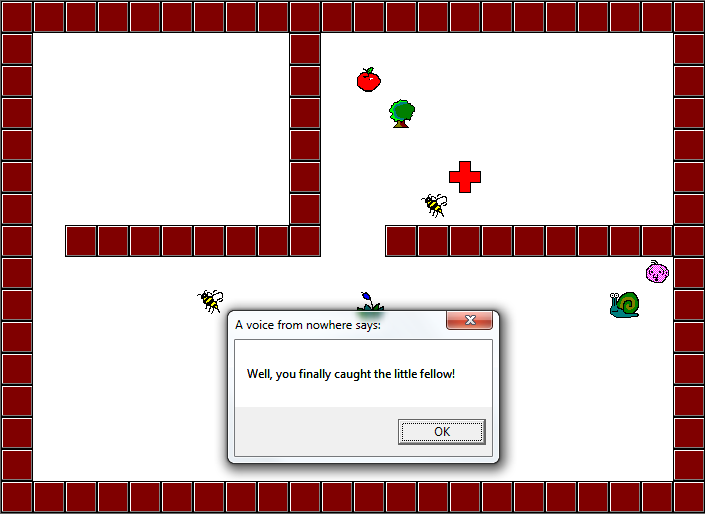
\includegraphics[width=0.5\textwidth]{bumbleBird1.png}
		\end{figure}


	The map bird one requires bumlbe to collect the birdseed and capture the bird whilst avoiding other agents on the map.  Generally bumble will survive this map 40 \% of the time, this success depends on several key features we have implemented in bumble. 
	
	Firstly is the issue of dealing with the wasps contained on the map, as these will attack bumble, these are also set to guard the bird seed. Bumble will generally avoid these hornets very well however quite often they will manage to damage him because of this it is essential bumble know the position of the heart and the tree so he can return to to these and recover, with out the mapping and search components this would not have been possible and bumble would have dropped off his mortal coil. 
	
	The snail presents a real issue to Bumble as it will often destroy his ability to search effectively because as it will follow him incessantly and get in his way, the snail can block bumble up against a wall causing him to starve to death, this is also an issue prevalent when the wasp and snail block Bumble in.

	
	\subsection{Test 1}
		Bumble will generally perfom well in this wolrd however this should be a given as there are a large amount of resources and a only one hornet to attack him, our perfomance with the current system is not as optimal as it has previously been where bumble could go infiniatly. To resolve the current issue with the system we feel that we need to improve the get closest method as this isn't actually giving and optimal goal. 
		
	\subsection{Test 2}
		The perfomance in this test is simalr to the the last test,  as bumble will now only survive a finite amount of time where he would previously 
		
		
		we belive that this isse has arise because the wasp is capable of holding bumble oagainst the wall and killing him
	
	
	
%\begin{table}[h!]
%	\centering
%	\begin{tabular}{| l | c | c | c | r |}
%	\hline
%		Map & Test 1 & Test 2 & Test 3 & Mean \\ \hline
%		Test 1 &  X & Y & Z & X+Y+Z/3 \\ \hline
%	\end{tabular}
%	\caption{This table shows some data}
%	\label{tab:myfirsttable}
%\end{table}

\section{Analysis}

What we found out from the results

\section{Conclusions}

\section{Further Work}

Although we were fairly pleased with the final outcome of the final game, there are a number of areas which could be improved upon and extended to provide an even more intelligent Bumble.
	
\subsection{Search Improvements}

At current the search in the system is simple in nature, it was desired to have implemented A* but this has unfortunately proven to be problematic.
		
The current search could be improved by searching for the same goal once a search is erased.
				
\subsection{Collision avoidance}
		
\subsection{Naturalistic search} 
		
\subsection{Mapping Improvements}

The mapping algorithm is simple in nature and could be improved by the use of? 
		
Boundary Detection (IE) can i see a wall ? is the cell adjacent a wall ? therefore i do not need to visit that cell because it won't reveal anymore information to me. 
	
The problem of mapping is strongly linked to Maze exploration, there are several interesting maze exploration algorithms such as (Azkaban algorithm, Dead-end filling, Wall follower ) and we feel that the use of one of these would make the Bumble's discovery of areas more effectively. 
	
		Out of these of  we feel that the wall follower algorithm is well suited to bumbles world would.... 
		
		Talk about wall follower.
		
\subsection{Objectives}

We could also add some sort of objectives system to the game to allow Bumble to actually plan his `method of attack'. Creating some basic rules which 

\subsection{Exploration}

\subsection{Machine Learning}

Another way that Bumble could be improved is by implementing machine learning techniques to allow him to develop a knowledgebase as he explores the world. Having both completed final year projects in this area, this is an area of great interest to us. The main factor holding us back was our inexperience using Prolog. 

Reinforcement learning's reward-punishment system would be particularly well suited to the VWorld environment; there could be various rewards given to Bumble for collecting items, catching the bird etc. Bumble could also be punished for pushing wasps and other dangerous objects. These rewards would encourage Bumble to perform well. Care would have to be taken to make sure that over-fitting doesn't occur (i.e. that Bumble doesn't learn lessons which are too specific to individual levels). The knowledge that Bumble develops would ideally be able to be applied to all levels.
		
\end{document}
